\documentclass[12pt]{article}
\usepackage{../../lecture_notes}
\usepackage{../../math}
\usepackage{../../uark_colors}


\title{Potential Outcomes}
\author{Prof. Kyle Butts}
\date{}

\hypersetup{
  colorlinks = true,
  allcolors = ozark_mountains,
  breaklinks = true,
  bookmarksopen = true
}

\begin{document}
\maketitle
\begin{multicols}{2}
\section*{Potential Outcomes Framework}

The potential outcomes framework, developed by Donald Rubin in a series of papers starting in 1974, provides a powerful way to think about causal relationships.
At its core, the framework asks us to imagine \emph{parallel universes} where the same unit experiences different treatments at exactly the same point in time.

Consider a policy intervention that affects some neighborhoods but not others.
For any given neighborhood $i$, we can imagine two potential outcomes:
\begin{itemize}
  \item $Y_i(1)$: the outcome for neighborhood $i$ \emph{in the parallel universe} where it receives the treatment
  \item $Y_i(0)$: the outcome for neighborhood $i$ \emph{in the parallel universe} where it does not receive treatment
\end{itemize}

The key insight is that these potential outcomes are characteristics of the unit itself, not dependent on what actually happens to other units.
Each neighborhood has both potential outcomes defined, regardless of which treatment it actually receives.

The \emph{unit-level causal effect} for neighborhood $i$ is simply the difference between these two potential outcomes:
$$\tau_i = Y_i(1) - Y_i(0)$$

This captures the causal impact of the treatment on that specific unit at that specific point in time.
Note that this is \emph{not} comparing the unit before and after treatment, but rather comparing two parallel states of the world for the same unit at the same moment.


Of course, estimating individual-level treatment effects is typically impossible due to noise and sample size constraints.
Instead, we focus on \emph{average} treatment effects that summarize impacts across groups of units.

The \emph{Average Treatment Effect} (ATE) averages the causal effect across all units in the population:
$$\tau_{\text{ATE}} = \expec{Y_i(1) - Y_i(0)}$$

Sometimes we care about the effect specifically for those who actually received treatment, called the \emph{Average Treatment Effect on the Treated} (ATT):
$$\tau_{\text{ATT}} = \expec{Y_i(1) - Y_i(0)}{D_i = 1}$$

We might also be interested in how treatment effects vary across different types of units.
The \emph{Conditional Average Treatment Effect} (CATE) summarizes the treatment effect for units with specific characteristics $\bm{X} = \bm{x}$:
$$\tau_{\text{CATE}}(x) = \expec{Y_i(1) - Y_i(0)}{\bm{X}_i = \bm{x}}$$

For example, we might ask: what is the effect of the policy intervention for neighborhoods with high income versus low income?
This allows us to understand treatment effect heterogeneity and target policies more effectively.

\section*{Causal Inference}

\begin{figure*}[!tb]
\centering
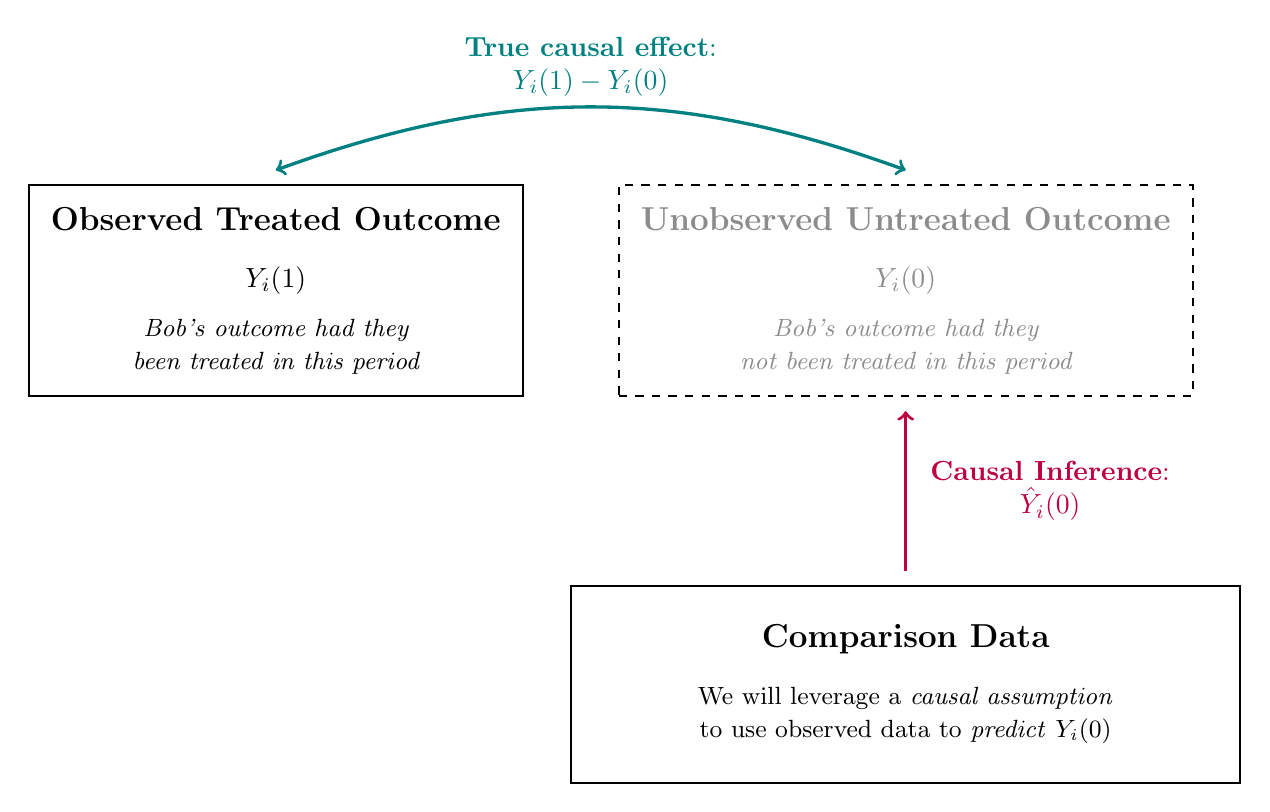
\begin{tikzpicture}[
  box/.style={draw, rectangle, minimum width=4cm, minimum height=2.5cm, align=center, inner sep=8pt},
  observed/.style={box, thick},
  unobserved/.style={box, dashed, thick, text=gray!90},
  comparison/.style={box, thick, minimum width=8.5cm}
]

% Top row - Potential outcomes
\node[observed] (treated) at (-4,5) {
  \textbf{\large Observed Treated Outcome} \\[0.3cm]
  $Y_i(1)$ \\[0.2cm]
  {\small\itshape Bob's outcome had they} \\
  {\small\itshape been treated in this period}
};

\node[unobserved] (untreated) at (4,5) {
  \textbf{\large Unobserved Untreated Outcome} \\[0.3cm]
  $Y_i(0)$ \\[0.2cm]
  {\small\itshape Bob's outcome had they} \\
  {\small\itshape not been treated in this period}
};

% Bottom row - Comparison data
\node[comparison] (comparison) at (4,0) {
  \textbf{\large Comparison Data} \\[0.3cm]

  {\small We will leverage a \emph{causal assumption}} \\
  {\small to use observed data to \emph{predict} $Y_i(0)$} %\\[0.4cm]
  % {\small - Similar untreated units} \\
  % {\small - Treated unit's data prior to treatment}
};

% Arrow between potential outcomes
\draw[<->, very thick, teal, bend left=20] 
  ([yshift=5pt]treated.north) to 
  node[midway, above, align=center] {
    \textbf{True causal effect}: \\ 
    $Y_i(1) - Y_i(0)$
  } 
  ([yshift=5pt]untreated.north);

% Arrow with label
\draw[->, very thick, purple] ([yshift=5pt]comparison.north) -- 
  node[midway, right, xshift=5pt, align=center] {
    \textbf{Causal Inference}: \\
    $\hat{Y}_i(0)$
  } ([yshift=-5pt]untreated.south);

\end{tikzpicture}

\caption{Potential Outcomes and Causal Inference}\label{fig:causal_inference}
\end{figure*}

Causal Inference is the study of how to identify the causal effects of some policy.
The `fundamental problem of causal inference' is that we can only observe one possible state of the world. 
If a unit is treated, we can only observe their \emph{treated} potential outcome, $Y_i(1)$.
If a unit is untreated, we can only observe their \emph{untreated} potential outcome, $Y_i(0)$.
To know the effect of a policy on an individual, we would need to observe \emph{both} potential outcomes. 
But, that would require us to view \emph{two parallel universes at the same point in time} which is of course not possible.

Instead, the method of Causal Inference is fundamentally about predicting the `missing counterfactual outcome' using observed data. 
In practice, this means using data on untreated observations to predict the untreated potential outcome for treated units (Figure \ref{fig:causal_inference}). 
This prediction is done using data on `similar' untreated individuals, using data for the treated individual prior to treatment, or a combination of both.



When we make this prediction of the missing potential outcome, we fundamentally are making a \emph{causal assumption}. 

This is a crucial leap of faith: we assume that the way we use data from a comparison group allows us to accurately predict what would have happened to the treated unit in the absence of treatment. 
This assumption is fundamentally untestable.
We can never observe the true counterfactual for any individual, so we can never verify whether our prediction is correct. 
\emph{All} causal inference methods rest on \emph{an unprovable assumption}.
We can assess its plausibility, but we can never prove it holds in any given case.\footnote{
  I am a big stickler on language here. 
  Do not ever say `prove'/`verify'/`confirm' the causal assumption.
  Instead, use words like `this gives us more confidence in'/`supports'/`alleviates concern' the causal assumption.
}


\section*{Randomized Controlled Trials}

The \emph{randomized controlled trial} (RCT) represents the `gold standard' for causal inference because it elegantly solves the fundamental problem of causal inference.
When treatment assignment is truly random, the comparison data becomes an excellent stand-in for the unobserved counterfactual.

In an RCT, each unit has some probability of being assigned to treatment, but this assignment is determined by a random process---like flipping a coin or drawing from a hat.
This randomization ensures that, \emph{on average}, the treated and control groups are identical in terms of all characteristics, both observed and unobserved.

Here's the key insight: when $D_i$ is randomly assigned, we have $(Y_i(0), Y_i(1)) \Perp D_i$.
This means that potential outcomes are independent of treatment assignment.
As a result, the average untreated potential outcome for the treated group equals the average untreated potential outcome for the control group:
$$\expec{Y_i(0)}{D_i = 1} = \expec{Y_i(0)}{D_i = 0}$$

This eliminates selection bias entirely.
The control group provides an unbiased estimate of what would have happened to the treated units in the absence of treatment.

With randomization, our comparison data directly gives us $\expec{Y_i(0)}{D_i = 0}$, which serves as our estimate for the missing counterfactual $\expec{Y_i(0)}{D_i = 1}$.
The difference-in-means estimator becomes:
\begin{align*}
  \hat{\tau} 
  &= \expec{Y_i}{D_i = 1} - \expec{Y_i}{D_i = 0} \\
  &= \expec{Y_i(1)}{D_i = 1} - \expec{Y_i(0)}{D_i = 0}
\end{align*}

Since randomization makes the treated and control groups comparable, this estimator provides an unbiased estimate of the Average Treatment Effect.
In fact, under randomization, the ATE, ATT, and ATC are all identical since the treatment and control groups are random samples from the same population.

This is why RCTs are so powerful: they transform the challenging problem of causal inference into a straightforward comparison of means between randomly assigned groups.
The randomization does the heavy lifting of ensuring that our comparison group is a valid counterfactual.

\section*{Selection Bias}

The fundamental problem of causal inference is that we can only observe one potential outcome for each unit.
While randomized controlled trials solve this problem elegantly, most empirical work in economics relies on observational data where treatment assignment is not random.
This creates a critical challenge: how do we estimate causal effects when units self-select into treatment based on their characteristics?

Consider our neighborhood apartment example again.
Developers don't randomly choose neighborhoods for new construction---they strategically select locations where they expect higher returns.
This means neighborhoods that receive new apartments likely differ systematically from those that don't, even before any apartment is built.

The naive approach would be to simply compare average outcomes between treated and untreated neighborhoods using the \emph{difference-in-means estimator}:
$$\hat{\tau}_{\text{DIM}} = \expec{Y_i}{D_i = 1} - \expec{Y_i}{D_i = 0}$$

But what does this estimator actually identify?
Using the switching equation $Y_i = Y_i(1)D_i + Y_i(0)(1-D_i)$, we can rewrite this as:
$$\hat{\tau}_{\text{DIM}} = \expec{Y_i(1)}{D_i = 1} - \expec{Y_i(0)}{D_i = 0}$$

To understand what this identifies, we can use the ``add and subtract'' trick by adding and subtracting $\expec{Y_i(0)}{D_i = 1}$:
\begin{align*}
\hat{\tau}_{\text{DIM}} &= \expec{Y_i(1)}{D_i = 1} - \expec{Y_i(0)}{D_i = 0} \\
&\quad\quad - \expec{Y_i(0)}{D_i = 1} + \expec{Y_i(0)}{D_i = 1} \\[0.5em]
&= \underbrace{\expec{Y_i(1) - Y_i(0)}{D_i = 1}}_{\text{ATT}} \\ 
&\quad\quad+ \underbrace{\expec{Y_i(0)}{D_i = 1} - \expec{Y_i(0)}{D_i = 0}}_{\text{Selection Bias}}
\end{align*}

The difference-in-means estimator equals the Average Treatment Effect on the Treated plus a \emph{selection bias} term.
This bias term captures the difference in average untreated potential outcomes between the treated and control groups.

\textbf{Selection bias} occurs when $\expec{Y_i(0)}{D_i = 1}$ $\neq\expec{Y_i(0)}{D_i = 0}$.
In our apartment example, this would mean that neighborhoods selected for new construction would have had different rent levels than other neighborhoods even if no apartments were built.
If developers target neighborhoods with rising demand (leading to higher counterfactual rents), the selection bias would be positive, making us overestimate the causal effect of new construction.

This bias is fundamentally untestable since we never observe $Y_i(0)$ for treated units.
We can assess its plausibility by examining whether treated and untreated units look similar on observable characteristics, but we can never verify our assumptions about unobservable differences.

The key insight is that selection bias arises whenever treatment assignment is correlated with potential outcomes.
This correlation can emerge through three main channels: selection based on expected treated outcomes $Y_i(1)$, selection based on expected untreated outcomes $Y_i(0)$, or selection based on expected gains $\tau_i$.
In observational studies, at least one of these is likely present, making causal identification challenging.

The remainder of this course focuses on research designs and econometric methods that help us address selection bias and credibly estimate causal effects from observational data.

\end{multicols}
\end{document}
